\documentclass[a4paper]{article}\usepackage[]{graphicx}\usepackage[]{xcolor}
% maxwidth is the original width if it is less than linewidth
% otherwise use linewidth (to make sure the graphics do not exceed the margin)
\makeatletter
\def\maxwidth{ %
  \ifdim\Gin@nat@width>\linewidth
    \linewidth
  \else
    \Gin@nat@width
  \fi
}
\makeatother

\definecolor{fgcolor}{rgb}{0.102, 0.102, 0.102}
\newcommand{\hlnum}[1]{\textcolor[rgb]{0.2,0.2,0.2}{#1}}%
\newcommand{\hlsng}[1]{\textcolor[rgb]{0.2,0.2,0.2}{#1}}%
\newcommand{\hlcom}[1]{\textcolor[rgb]{0.302,0.302,0.302}{\textit{#1}}}%
\newcommand{\hlopt}[1]{\textcolor[rgb]{0.102,0.102,0.102}{#1}}%
\newcommand{\hldef}[1]{\textcolor[rgb]{0.102,0.102,0.102}{#1}}%
\newcommand{\hlkwa}[1]{\textcolor[rgb]{0.102,0.102,0.102}{#1}}%
\newcommand{\hlkwb}[1]{\textcolor[rgb]{0.102,0.102,0.102}{#1}}%
\newcommand{\hlkwc}[1]{\textcolor[rgb]{0.2,0.2,0.2}{#1}}%
\newcommand{\hlkwd}[1]{\textcolor[rgb]{0.102,0.102,0.102}{\textbf{#1}}}%
\let\hlipl\hlkwb

\usepackage{framed}
\makeatletter
\newenvironment{kframe}{%
 \def\at@end@of@kframe{}%
 \ifinner\ifhmode%
  \def\at@end@of@kframe{\end{minipage}}%
  \begin{minipage}{\columnwidth}%
 \fi\fi%
 \def\FrameCommand##1{\hskip\@totalleftmargin \hskip-\fboxsep
 \colorbox{shadecolor}{##1}\hskip-\fboxsep
     % There is no \\@totalrightmargin, so:
     \hskip-\linewidth \hskip-\@totalleftmargin \hskip\columnwidth}%
 \MakeFramed {\advance\hsize-\width
   \@totalleftmargin\z@ \linewidth\hsize
   \@setminipage}}%
 {\par\unskip\endMakeFramed%
 \at@end@of@kframe}
\makeatother

\definecolor{shadecolor}{rgb}{.97, .97, .97}
\definecolor{messagecolor}{rgb}{0, 0, 0}
\definecolor{warningcolor}{rgb}{1, 0, 1}
\definecolor{errorcolor}{rgb}{1, 0, 0}
\newenvironment{knitrout}{}{} % an empty environment to be redefined in TeX

\usepackage{alltt}

\usepackage{Rd}

% Definitions
\newcommand{\slan}{{\sffamily S}}
\newcommand{\rlan}{{\sffamily R}}
\newcommand{\grid}{\pkg{grid}}
\newcommand{\responseRateAnalysis}{\pkg{responseRateAnalysis}}
\newcommand{\lattice}{\CRANpkg{lattice}}

\newcommand{\todo}[1]{\textcolor{red}{TODO: #1}}
\newcommand{\note}[1]{\textcolor{blue}{NOTE: #1}}

\setlength{\parindent}{0in}
\setlength{\parskip}{.1in}
\setlength{\textwidth}{140mm}
\setlength{\oddsidemargin}{10mm}

% Packages
\usepackage{natbib}
\usepackage{xcolor}
\usepackage{graphicx}
\usepackage{hyperref}
\usepackage[capitalize]{cleveref}
\usepackage{enumitem}
\usepackage{adjustbox}
\usepackage{multicol}
\usepackage[ruled]{algorithm2e}
\usepackage{amssymb}

% kableExtra
\usepackage{booktabs}
\usepackage{longtable}
\usepackage{array}
\usepackage{multirow}
\usepackage{wrapfig}
\usepackage{float}
\usepackage{colortbl}
\usepackage{pdflscape}
\usepackage{tabu}
\usepackage{threeparttable}
\usepackage{threeparttablex}
\usepackage[normalem]{ulem}
\usepackage{makecell}
\usepackage{xcolor}

% Citation style
\bibliographystyle{ivt-style/ivt-eng}

\title{Predicting response rates once again}
\author{Daniel Heimgartner \& Kay W. Axhausen}
\IfFileExists{upquote.sty}{\usepackage{upquote}}{}
\begin{document}

\maketitle









% !Rnw root = paper.Rnw



\section{Introduction}

Counting \textit{response burden scores} \citep{schmid2019predicting} is not a very popular task at the Institute for Transport Planning and Systems (IVT, ETH Zurich). One or the other former PhD student got away without reporting them. However, the collective effort over the years yielded a unique dataset allowing us to understand response rates as a function of recruitment efforts and incentives. Other research institutes would therefore be encouraged to also contribute (despite the burden of counting response burden). This paper briefly elaborates the methodology once again and introduces the \responseRateAnalysis~\rlan-package (\url{https://github.com/dheimgartner/responseRateAnalysis}) with its helper functions to easily replicate the results. Since the last update \citep{axhausen2019predicting} a handful exemplary students got their PhD and left not until the last response burden score of their surveys was counted. Thanks to them, we feel that the time is right to predict response rates once again.

The package can be installed as elaborated below but we hope that other research groups rather clone the repository and contribute with their scored survey instruments according to the guidelines outlined on github so that we or they can predict response rates from time to time again. The tutorial nature of this report will hopefully make this no burden whatsoever.

\begin{knitrout}
\definecolor{shadecolor}{rgb}{1, 1, 1}\color{fgcolor}\begin{kframe}
\begin{alltt}
\hldef{> }\hldef{devtools}\hlopt{::}\hlkwd{install_github}\hldef{(}\hlsng{"dheimgartner/responseRateAnalyis"}\hldef{)}
\end{alltt}
\end{kframe}
\end{knitrout}

\note{"Last publication" refers to the \citet{axhausen2019predicting}. The journal publication \citep{schmid2019predicting} is based on only N=47 (see table 3)... But the surveys listed in table 2 contain 65 surveys?? There is something a little weird there.}

\section{Data}

The main data collection effort consists of scoring the survey instruments according to \cref{tab:response_burden_scheme}.



\begin{table}

\caption{\label{tab:response_burden_scheme}Response burden: Points by question type and action}
\centering
\begin{tabular}[t]{lr}
\toprule
Item & Points\\
\midrule
Question or transition (up to 3 lines) & 2.0\\
\hspace{2em}Each additional line & 1.0\\
Closed yes/no answers & 1.0\\
Simple numerical answer (e.g., year of birth) & 1.0\\
Rating with up to 5 possibilities & 2.0\\
\addlinespace
Rating with more than 5 possibilties & 3.0\\
Left, middle, right rating & 2.0\\
Scales with 3 and more grades & 2.0\\
Best of ranking with cards & 4.0\\
\hspace{2em}Second and each additional best ranking & 3.0\\
\addlinespace
Answer to sub-questions of up to 5 words & 1.0\\
Answer to sub-question of up to 2 lines & 2.0\\
a) Rsponse to half-open question with less than 8 possibilities & 2.0\\
\hspace{2em}Each additional one & 2.0\\
b) Response to half-open question with at least 8 possibilities & 4.0\\
\addlinespace
\hspace{2em}Each additional one & 3.0\\
Answer to "please specify" & 2.0\\
First answer to an open question & 6.0\\
\hspace{2em}Each additional answer to the open question & 3.0\\
Mixing showcards & 6.0\\
\addlinespace
Giving/showing a card to the respondent & 1.0\\
\hspace{2em}Per response category on a showcard & 1.0\\
Filter & 0.5\\
Branching & 0.5\\
For each stated choice question with 2 alternatives & 2.0\\
\addlinespace
For each stated choice question with 3 alternatives & 3.0\\
For each variable of the stated choice situation and each question & 1.0\\
\bottomrule
\multicolumn{2}{l}{\rule{0pt}{1em}Based on \textit{Gesellschaft für Sozialforschung (GfS)}, Zürich, 2006 (updated).}\\
\end{tabular}
\end{table}



In comparison to the previous publication \citep{schmid2019predicting}, 14 additional surveys were added by IVT members. A new group (no recruitment but with incentive payments) is now part of the sample. However, only five studies fall in this category. The current state of the database is attached to the package \code{response\_rates} and its variables documented (\code{?response\_rates}). The full sample underlying this report can be found in \cref{tab:full_sample}.

The distribution of the response burden scores (RBS) for the four recruitment and incentive categories are visualized in \cref{fig:response_burden_scores}. The median RBS is 399 and surveys with a score higher than 1`500 are rare (twelve points roughly correspond to a one-minute response time).

\begin{figure}
\begin{knitrout}
\definecolor{shadecolor}{rgb}{1, 1, 1}\color{fgcolor}

{\centering 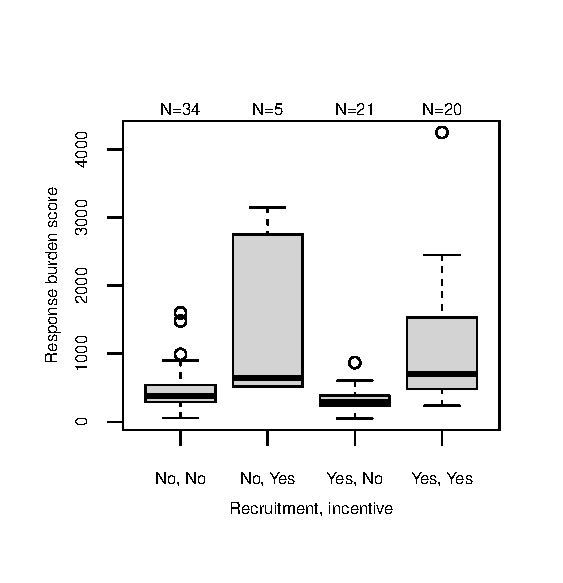
\includegraphics[width=0.5\linewidth]{figure/unnamed-chunk-14-1} 

}


\end{knitrout}
\caption{Distribution of the response burden scores for \textit{recruitment x intentive} categories.}
\label{fig:response_burden_scores}
\end{figure}

\section{Methods}

Building on \citet{axhausen2019predicting}, we estimate a logistic regression model relating response burden scores to log-transformed response rates:

\begin{equation}
\log \left( \frac{y_i}{100 - y_i} \right) = \beta_0 + \beta_1 \frac{x_i}{1000} + \varepsilon_i
\label{eq:response_burden}
\end{equation}

where $y_i$ denotes the response rate (in percent), $x_i$ represents the ex-ante response burden score, and $\varepsilon_i$ is a normally distributed clustered error term (similar errors for different survey waves of the same study). Observations were weighted by the square root of the sample size. The model was estimated for the entire sample (excluding surveys with a sample size less than ten) as well as separately for recruitment by incentive category. The exponential $\exp(\beta_1)$ represents a marginal change in odds ratio (i.e., participation vs. non-participation).

If a survey instrument's response burden score increases by 100 points, the odds of participating decrease according to:

\begin{equation}
\left( \exp \left( \frac{\beta_1}{1000} \right) -1 \right) \cdot 100
\label{eq:log_odds_decrease}
\end{equation}

\section{Results}

The basic workflow is as follows:

\begin{enumerate}
\item \code{default\_data()} loads and prepares the \code{response\_rates} data for estimation. It selects the input variables, computes the weights (\code{sqrt(sample\_size)}), rescales the response burden score (\code{response\_burden\_score / 1000}) and log transforms the response rate (\code{log(response\_rate / (100 - response\_rate))}).
\item Fit a linear regression model with \code{lm}.
\item Add clustered standard errors with \code{add\_clustered()} which uses the \pkg{clubSandwich} \citep{clubsandwich} and \pkg{lmtest} package \citep{lmtest} under the hood to correct standard errors and related statistics.
\end{enumerate}

The following code conducts the analysis for the full sample (i.e., same slope but different intercepts for the \textit{recruitment x incentive} category), where the category recruited and incentives paid (\textit{yes, yes}) serves as the reference:

\begin{knitrout}
\definecolor{shadecolor}{rgb}{1, 1, 1}\color{fgcolor}\begin{kframe}
\begin{alltt}
\hldef{> }\hldef{dat} \hlkwb{<-} \hlkwd{default_data}\hldef{()} \hlopt
\hldef{+ }  \hlkwd{filter}\hldef{(sample_size} \hlopt{>=} \hlnum{10}\hldef{)}  \hlcom{# to be consistent with previous publications}
\hldef{> }\hldef{fit} \hlkwb{<-} \hlkwd{lm}\hldef{(y} \hlopt{~} \hlnum{0} \hlopt{+} \hldef{x} \hlopt{+} \hldef{yes_no} \hlopt{+} \hldef{no_no} \hlopt{+} \hldef{no_yes,}  \hlcom{# yes_yes is the reference}
\hldef{+ }          \hlkwc{data} \hldef{= dat,} \hlkwc{weights} \hldef{= weight)}
\hldef{> }\hldef{m1} \hlkwb{<-} \hlkwd{add_clustered}\hldef{(fit,} \hlkwc{cluster} \hldef{= dat}\hlopt{$}\hldef{survey_id,} \hlkwc{type} \hldef{=} \hlsng{"CR2"}\hldef{)}
\hldef{> }\hlkwd{class}\hldef{(m1)}
\end{alltt}
\begin{verbatim}
[1] "clustered" "lm"       
\end{verbatim}
\end{kframe}
\end{knitrout}

The functions from the \pkg{texreg} \citep{texreg} package (e.g., \code{screenreg()} or \code{texreg()}) work together with the class \code{"clustered" "lm"} and produce the tables reported in this work.

We repeat the above estimation for different samples, comparing the estimates of the last publication to the updated ones as well as estimate separate models for the four different recruitment and incentive categories. \cref{tab:comparison} summarises the results.

\note{In \citet{schmid2019predicting} you did include a dummy for all three categories in the pooled model (why no reference?).}




\begin{table}
\caption{Logistic regression results: Regressing response burden score on (logit-transformed) response rates}
\begin{center}
\scalebox{0.75}{
\begin{tabular}{l c c c c c c c c c}
\toprule
 & \multicolumn{5}{c}{Updated models} & \multicolumn{4}{c}{Old models\dag} \\
\cmidrule(lr){2-6} \cmidrule(lr){7-10}
 & Pooled & Yes, yes & Yes, no & No, no & No, yes & Pooled & Yes, yes & Yes, no & No, no \\
\midrule
Response burden & $-0.53$     & $-0.31^{**}$ & $-2.97^{***}$ & $-1.63^{**}$ & $-1.05$  & $0.24$        & $-0.32^{**}$ & $-1.55$     & $-1.25^{***}$ \\
                & $(0.50)$    & $(0.11)$     & $(0.72)$      & $(0.47)$     & $(0.40)$ & $(0.19)$      & $(0.11)$     & $(1.16)$    & $(0.31)$      \\
Yes, no         & $0.41$      &              &               &              &          & $0.59^{***}$  &              &             &               \\
                & $(0.45)$    &              &               &              &          & $(0.16)$      &              &             &               \\
No, no          & $-0.84^{*}$ &              &               &              &          & $-1.48^{***}$ &              &             &               \\
                & $(0.39)$    &              &               &              &          & $(0.22)$      &              &             &               \\
No, yes         & $-1.77^{*}$ &              &               &              &          &               &              &             &               \\
                & $(0.84)$    &              &               &              &          &               &              &             &               \\
Intercept       &             & $1.23^{***}$ & $1.49^{***}$  & $-0.38$      & $-0.64$  &               & $1.25^{***}$ & $1.13^{**}$ & $-0.81^{***}$ \\
                &             & $(0.16)$     & $(0.26)$      & $(0.41)$     & $(0.74)$ &               & $(0.18)$     & $(0.32)$    & $(0.20)$      \\
\midrule
R$^2$           & $0.70$      & $0.13$       & $0.71$        & $0.16$       & $0.92$   & $0.68$        & $0.13$       & $0.13$      & $0.22$        \\
Adj. R$^2$      & $0.68$      & $0.08$       & $0.70$        & $0.13$       & $0.90$   & $0.66$        & $0.08$       & $0.07$      & $0.19$        \\
Num. obs.       & $79$        & $20$         & $20$          & $34$         & $5$      & $67$          & $19$         & $18$        & $30$          \\
LL              & $-122.58$   & $-20.97$     & $-15.51$      & $-47.70$     & $-2.48$  & $-84.67$      & $-20.75$     & $-13.94$    & $-31.10$      \\
AIC             & $255.17$    & $47.94$      & $37.02$       & $101.39$     & $10.97$  & $177.33$      & $47.49$      & $33.89$     & $68.20$       \\
BIC             & $267.02$    & $50.92$      & $40.00$       & $105.97$     & $9.80$   & $186.15$      & $50.33$      & $36.56$     & $72.40$       \\
\bottomrule
\multicolumn{10}{l}{\scriptsize{$^{***}p<0.001$; $^{**}p<0.01$; $^{*}p<0.05$. \dag Based on the sample of the last publication.}}
\end{tabular}
}
\label{tab:comparison}
\end{center}
\end{table}


For the newly added group (no recruitment but with incentive payments, \textit{no, yes}) the effect of the response burden is not significant, as expected because of limited sample size. Due to the logistic transformation, parameters reflect changes in log-odds when the RBS marginally increases. The effect of response burden is generally more negative than previously expected. The strongest effect can be found for the recruited subsample without incentive payment (\textit{yes, no}), where the odds of participating decrease by -0.297 (i.e., roughly 30\%) according to \cref{eq:log_odds_decrease} if the RBS increases by 100 points. The other comparisons are listed in \cref{tab:pc_odds}.



\begin{table}
\centering
\caption{\label{tab:pc_odds}Percentage change in the odds of participating if the response burden score increases by 100 points}
\centering
\fontsize{9}{11}\selectfont
\begin{tabular}[t]{lrr}
\toprule
Category & Updated models [\%] & Old models [\%]\\
\midrule
Pooled & -5.26 & 2.42\\
Yes, yes & -3.13 & -3.23\\
Yes, no & -29.66 & -15.50\\
No, no & -16.30 & -12.46\\
No, yes & -10.51 & \\
\bottomrule
\end{tabular}
\end{table}



\begin{figure}[h!]
\begin{knitrout}
\definecolor{shadecolor}{rgb}{1, 1, 1}\color{fgcolor}

{\centering 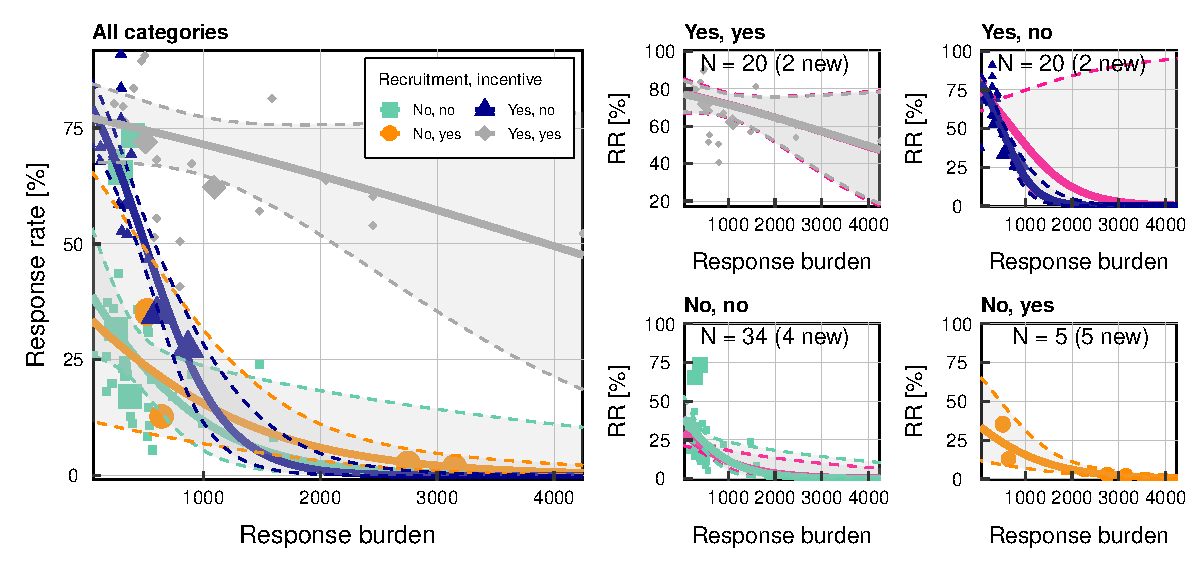
\includegraphics[width=\maxwidth]{figure/unnamed-chunk-20-1} 

}


\end{knitrout}
\caption{Response rate curves (response rates as a function of the response burden). The left-hand panel compares the curves for each \textit{recruitment x incentive} category based on the four separately estimated models. The right-hand (smaller) panels compare the response rate curves to the ones based on the data of the previous publication (pink lines). New data points (since the last publication) are enlarged.}
\label{fig:response_curves}
\end{figure}

The back-transformed relationship between response burden and response rates (response rate curve) is visualized in \cref{fig:response_curves}, along their confidence intervals (i.e., the shaded area reflects the uncertainty of the curve estimates and is not a prediction interval). Recruitment shifts the curve, while incentives flatten it. Notably, the domain above a response burden score of 2`000 is sparsely populated, and the few observations potentially strongly influence the curve's shape (however, according to \textit{Cook's distance} no influential outliers are present in our data). The results indicate that surveys beyond 2`000 points appear overly burdensome for respondents, sustaining high response rates only through recruitment efforts combined with incentive payments, intensive care of the respondents and general interest in the topic of these intense studies.

Generally, the 14 new data points do not dramatically change the overall shape of the curves (\cref{fig:response_curves}, RHS), but the curves are slightly steeper as explained based on the parameter estimates. \textit{Yes, yes} is almost identical (only two new data points were added). For \textit{no, no} the confidence bounds increased because two of the five added surveys have unprecedented high response rates. For the category \textit{yes, no} the function has gained support for higher response burdens which substantially steepened the curve and reduced its uncertainty. In particular, we now have higher confidence that the curve quickly joins the other response curves on the domain above 1`500 response burden points. I.e., recruitment without incentive payments only matters for surveys with low response burden (but can make a big difference there).

\subsection*{Adding a linear time-trend}

Similar to \citet{schmid2019predicting}, we can add a linear time-trend with the year 2004 (when the survey scoring effort started) serving as the base. The following code shows the trivial addition of the time-trend to the pooled model.

\begin{knitrout}
\definecolor{shadecolor}{rgb}{1, 1, 1}\color{fgcolor}\begin{kframe}
\begin{alltt}
\hldef{> }\hldef{dat}\hlopt{$}\hldef{year} \hlkwb{<-} \hldef{dat}\hlopt{$}\hldef{year} \hlopt{-} \hlnum{2004}
\hldef{> }
\hldef{> }\hldef{fit_t} \hlkwb{<-} \hldef{fit_t} \hlkwb{<-} \hlkwd{lm}\hldef{(y} \hlopt{~} \hlnum{0} \hlopt{+} \hldef{x} \hlopt{+} \hldef{yes_no} \hlopt{+} \hldef{no_no} \hlopt{+} \hldef{no_yes} \hlopt{+} \hldef{year,}
\hldef{+ }                     \hlkwc{data} \hldef{= dat,} \hlkwc{weights} \hldef{= weight)}
\hldef{> }
\hldef{> }\hldef{mt} \hlkwb{<-} \hlkwd{add_clustered}\hldef{(fit_t,} \hlkwc{cluster} \hldef{= dat}\hlopt{$}\hldef{survey_id,} \hlkwc{type} \hldef{=} \hlsng{"CR2"}\hldef{)}
\end{alltt}
\end{kframe}
\end{knitrout}

We repeat the steps for the individual categories and synthesise the results in a table (\cref{tab:time_trend}). In contrast to \citet{schmid2019predicting} we do not find a negative time-trend and therefore do not support the hypothesis of a general fatigue and less willingness to participate in our surveys.




\begin{table}
\caption{Logistic regression results: Adding a linear time-trend}
\begin{center}
\scalebox{0.72}{
\begin{tabular}{l c c c c c c c c c c}
\toprule
 & \multicolumn{5}{c}{No time-trend} & \multicolumn{5}{c}{With time-trend} \\
\cmidrule(lr){2-6} \cmidrule(lr){7-11}
 & Pooled & Yes, yes & Yes, no & No, no & No, yes & Pooled & Yes, yes & Yes, no & No, no & No, yes \\
\midrule
Response burden & $-0.53$     & $-0.31^{**}$ & $-2.97^{***}$ & $-1.63^{**}$ & $-1.05$  & $-0.68$       & $-0.33^{*}$ & $-3.28^{**}$ & $-1.50^{**}$ & $-1.41^{*}$ \\
                & $(0.50)$    & $(0.11)$     & $(0.72)$      & $(0.47)$     & $(0.40)$ & $(0.44)$      & $(0.13)$    & $(0.85)$     & $(0.44)$     & $(0.24)$    \\
Yes, no         & $0.41$      &              &               &              &          & $0.01$        &             &              &              &             \\
                & $(0.45)$    &              &               &              &          & $(0.56)$      &             &              &              &             \\
No, no          & $-0.84^{*}$ &              &               &              &          & $-1.25^{***}$ &             &              &              &             \\
                & $(0.39)$    &              &               &              &          & $(0.35)$      &             &              &              &             \\
No, yes         & $-1.77^{*}$ &              &               &              &          & $-2.33^{**}$  &             &              &              &             \\
                & $(0.84)$    &              &               &              &          & $(0.79)$      &             &              &              &             \\
Intercept       &             & $1.23^{***}$ & $1.49^{***}$  & $-0.38$      & $-0.64$  &               & $1.06^{*}$  & $1.49^{***}$ & $-0.71^{*}$  & $-12.31$    \\
                &             & $(0.16)$     & $(0.26)$      & $(0.41)$     & $(0.74)$ &               & $(0.43)$    & $(0.32)$     & $(0.34)$     & $(8.03)$    \\
Time-trend      &             &              &               &              &          & $0.05^{*}$    & $0.02$      & $0.01$       & $0.03$       & $0.68$      \\
                &             &              &               &              &          & $(0.02)$      & $(0.05)$    & $(0.06)$     & $(0.05)$     & $(0.46)$    \\
\midrule
R$^2$           & $0.70$      & $0.13$       & $0.71$        & $0.16$       & $0.92$   & $0.73$        & $0.14$      & $0.72$       & $0.20$       & $0.97$      \\
Adj. R$^2$      & $0.68$      & $0.08$       & $0.70$        & $0.13$       & $0.90$   & $0.71$        & $0.04$      & $0.68$       & $0.14$       & $0.95$      \\
Num. obs.       & $79$        & $20$         & $20$          & $34$         & $5$      & $79$          & $20$        & $20$         & $34$         & $5$         \\
LL              & $-122.58$   & $-20.97$     & $-15.51$      & $-47.70$     & $-2.48$  & $-118.55$     & $-20.81$    & $-15.38$     & $-46.95$     & $0.06$      \\
AIC             & $255.17$    & $47.94$      & $37.02$       & $101.39$     & $10.97$  & $249.09$      & $49.61$     & $38.76$      & $101.89$     & $7.89$      \\
BIC             & $267.02$    & $50.92$      & $40.00$       & $105.97$     & $9.80$   & $263.31$      & $53.59$     & $42.74$      & $108.00$     & $6.33$      \\
\bottomrule
\multicolumn{11}{l}{\scriptsize{$^{***}p<0.001$; $^{**}p<0.01$; $^{*}p<0.05$.}}
\end{tabular}
}
\label{tab:time_trend}
\end{center}
\end{table}


\section{Limitations and future research}

\begin{itemize}
\item Response burden scores should be treated as random (i.e., feature measurement errors) since the assignment of response burden scores according to \cref{tab:response_burden_scheme} is not always clear. The modeling approach would need to be adjusted accordingly.
\item The form and value of the incentive should be considered (currently we only know whether or not an incentive had been paid).
\item While we checked for influential data points consulting \textit{Cook's distance} (which did not indicate any outliers), there are only few observations with response burden scores higher than 2`000 points.
\item We hope that other research groups join the effort to collect response burden scores such that our insights can be generalized to other institutions, domains and countries.
\end{itemize}


% Bibliography
\clearpage
\bibliography{bib/references}

% Appendix
\clearpage
\appendix

% !Rnw root = paper.Rnw



\section{Full data sample}
\label{appendix}

\begin{knitrout}
\definecolor{shadecolor}{rgb}{1, 1, 1}\color{fgcolor}\begin{kframe}
\begin{alltt}
\hldef{> }\hldef{rr} \hlkwb{<-}
\hldef{+ }  \hldef{response_rates} \hlopt
\hldef{+ }  \hlkwd{select}\hldef{(year, survey_content, sample_size, response_burden_score, response_rate)}
\hldef{> }
\hldef{> }\hlkwd{names}\hldef{(rr)} \hlkwb{<-} \hlkwd{c}\hldef{(}\hlsng{"Year"}\hldef{,} \hlsng{"Study"}\hldef{,} \hlsng{"Sample size"}\hldef{,} \hlsng{"Burden score"}\hldef{,}
\hldef{+ }               \hlsng{"Response rate [%]"}\hldef{)}
\hldef{> }
\hldef{> }\hldef{tex} \hlkwb{<-} \hldef{kableExtra}\hlopt{::}\hlkwd{kbl}\hldef{(rr,} \hlkwc{format} \hldef{=} \hlsng{"latex"}\hldef{,}
\hldef{+ }                       \hlkwc{caption} \hldef{=} \hlsng{"Updated response burden scores"}\hldef{,}
\hldef{+ }                       \hlkwc{label} \hldef{=} \hlsng{"full_sample"}\hldef{,} \hlkwc{digits} \hldef{=} \hlnum{0}\hldef{,}
\hldef{+ }                       \hlkwc{longtable} \hldef{=} \hlnum{TRUE}\hldef{,}
\hldef{+ }                       \hlkwc{booktabs} \hldef{=} \hlnum{TRUE}\hldef{)} \hlopt
\hldef{+ }  \hldef{kableExtra}\hlopt{::}\hlkwd{kable_styling}\hldef{(}\hlkwc{latex_options} \hldef{=} \hlkwd{c}\hldef{(}\hlsng{"repeat_header"}\hldef{))} \hlopt
\hldef{+ }  \hldef{kableExtra}\hlopt{::}\hlkwd{landscape}\hldef{()}
\end{alltt}
\end{kframe}
\end{knitrout}


\begin{landscape}
\begin{longtable}[t]{rlrrr}
\caption{\label{tab:full_sample}Updated response burden scores}\\
\toprule
Year & Study & Sample size & Burden score & Response rate [\%]\\
\midrule
\endfirsthead
\caption[]{Updated response burden scores \textit{(continued)}}\\
\toprule
Year & Study & Sample size & Burden score & Response rate [\%]\\
\midrule
\endhead

\endfoot
\bottomrule
\endlastfoot
2004 & National SP survey on railway services & 1561 & 120 & 68\\
2006 & Regional mode and route choice SP & 1229 & 120 & 71\\
2007 & National SP on value of travel time savings & 2317 & 303 & 53\\
2004 & Regional SR on value of statistical life & 500 & 440 & 36\\
2006 & Regional SR on value of statistical life & 1900 & 526 & 31\\
\addlinespace
2005 & Home ownership and use of local facilities & 9330 & 231 & 36\\
2007 & National SP on the impacts of road pricing & 2227 & 524 & 47\\
2005 & Mobility biographies and regular travel & 3290 & 521 & 8\\
2005 & Mobility biographies & 1645 & 529 & 31\\
2005 & Mobility biographies & 1435 & 529 & 15\\
\addlinespace
2004 & Mobility biographies and home ownership & 297 & 655 & 20\\
2006 & Social network and mobility biographies & 2714 & 992 & 11\\
2008 & Mobility Plan University & 363 & 219 & 20\\
2008 & Mobility Plan USZ & 1615 & 57 & 26\\
2009 & Fuel price and rail usage & 993 & 327 & 58\\
\addlinespace
2009 & Modelling mountaineers' travel behaviour & 530 & 276 & 44\\
2009 & Snowball sample & 826 & 900 & 67\\
2009 & Snowball sample & 312 & 900 & 22\\
2009 & Snowball sample & 142 & 1480 & 57\\
2010 & Snowball sample & 50 & 1480 & 24\\
\addlinespace
2010 & Diary induced traffic, pen-and-paper & 200 & 800 & 50\\
2010 & Diary induced traffic, online & 140 & 800 & 41\\
2010 & 2000 Watt society, pretest 1 & 51 & 326 & 76\\
2010 & 2000 Watt society, pretest 2 & 49 & 314 & 80\\
2010 & 2000 Watt society, main study & 491 & 238 & 80\\
\addlinespace
2010 & ARE SP, pretest - mode choice only & 99 & 235 & 69\\
2010 & ARE SP, pretest - route choice only & 29 & 280 & 59\\
2010 & ARE SP, pretest - mode and route choice & 484 & 384 & 72\\
2010 & ARE SP, main study - mode choice only & 893 & 235 & 69\\
2010 & ARE SP, main study - route choice only & 215 & 280 & 67\\
\addlinespace
2010 & ARE SP, main study - mode and route choice & 3994 & 384 & 69\\
2011 & Residential choice (Otte, no addresses) & 1200 & 320 & 25\\
2011 & Residential choice (Otte, with addresses) & 1200 & 330 & 21\\
2011 & Residential choice (Own items, no addresses) & 1200 & 344 & 24\\
2011 & Residential choice (Own items, with addresses) & 1200 & 354 & 22\\
\addlinespace
2011 & Grimsel user SP & 399 & 180 & 71\\
2011 & Survey on bus and tram use & 3177 & 310 & 23\\
2011 & Survey on parking behaviour & 1248 & 404 & 84\\
2012 & SP survey on travel time reliability & 491 & 400 & 73\\
2011 & BABS SC (Evacuation) & 4049 & 330 & 25\\
\addlinespace
2012 & Car sharing / pooling & 1683 & 350 & 52\\
2012 & BMVBS Zeitkosten, schriftlich & 3355 & 600 & 68\\
2012 & BMVBS Zeitkosten, online & 209 & 600 & 56\\
2012 & BMVBS Zeitkosten, gewerblich & 925 & 500 & 91\\
2012 & Climate Change Influence on Swiss Transport - Interviews & 16 & 48 & 38\\
\addlinespace
2013 & Climate Change Influence on Swiss Transport - Written Questionnaire & 5 & 165 & 80\\
2013 & Mobility Biographies & 288 & 1600 & 8\\
2014 & Climate Change Influence on Swiss Transport - Online Questionnaire & 55 & 168 & 18\\
2014 & Mobility-Pilotprojekts zu free-floating Carsharing - Mobility-Kunden & 2224 & 173 & 26\\
2014 & Mobility-Pilotprojekts zu free-floating Carsharing - Catch a Car-Kunden & 527 & 178 & 37\\
\addlinespace
2014 & Masterarbeit Verkehr und Soziale Netzwerke & 208 & 580 & 51\\
2015 & Masterarbeit Arbeitsplatzwahl (freie Wahl einer Arbeitsstelle) & 265 & 290 & 69\\
2015 & Masterarbeit Arbeitsplatzwahl (Wechsel der Arbeitsstelle) & 11 & 296 & 91\\
2015 & Masterarbeit Arbeitsplatzwahl (Wechsel der Arbeitsstelle) & 140 & 296 & 84\\
2015 & ARE SP 2015 & 6099 & 296 & 77\\
\addlinespace
2015 & Post-Car World (Pre-Test: Stage 1,2,3) & 67 & 4250 & 52\\
2015 & Post-Car World (Wave 1: Stage 1,2,3) & 137 & 2450 & 54\\
2015 & Post-Car World (Wave 2: Stage 1,2,3) & 191 & 2451 & 60\\
2016 & Post-Car World (Wave 3: Stage 1,2) & 118 & 2050 & 64\\
2017 & Pretest: Social Networks, Mobility Behaviour and Societal Impacts (1st survey part) & 500 & 740 & 17\\
\addlinespace
2017 & Pretest: Social Networks, Mobility Behaviour and Societal Impacts (2nd survey part) & 57 & 470 & 89\\
2017 & Social Networks, Mobility Behaviour and Societal Impacts (1st survey part) & 12000 & 553 & 21\\
2017 & Social Networks, Mobility Behaviour and Societal Impacts (2nd survey part) & 1706 & 1588 & 81\\
2018 & SVI (pretest): Einfluss nicht verkehrlicher Variablen: Neuzuzüger & 241 & 540 & 11\\
2018 & SVI (pretest): Einfluss nicht verkehrlicher Variablen: Eingesessene & 252 & 378 & 13\\
\addlinespace
2018 & SVI (main survey):  Einfluss nicht verkehrlicher Variablen: Neuzuzüger & 4825 & 568 & 6\\
2018 & SVI (main survey): Einfluss nicht verkehrlicher Variablen: Eingesessene & 4601 & 396 & 11\\
2017 & Automated Vehicles main study (Stage 1,2,3) & 482 & 1092 & 62\\
2021 & Kontext: Yumuv. Inhalte: Haushalt, Verkehrsmittel. & 10000 & 643 & 13\\
2022 & Swiss Value of time study (pre-test \& wave 1) & 2545 & 520 & 36\\
\addlinespace
2022 & Swiss Value of time study (wave 2) & 2548 & 520 & 35\\
2020 & Swiss Mobility Panel Wave 1 & 27417 & 604 & 35\\
2021 & Swiss Mobility Panel Wave 2 & 9442 & 398 & 73\\
2022 & Swiss Mobility Panel Wave 3 & 9092 & 290 & 65\\
2022 & Swiss Mobility Panel Wave 4 (sample refresh) & 11000 & 869 & 27\\
\addlinespace
2022 & TimeusePlus (pre-test) & 7500 & 2750 & 3\\
2023 & TimeusePlus (main study) & 69000 & 3150 & 2\\
2022 & Multimodality in the Swiss New Normal (SNN): Pre-study & 7876 & 373 & 17\\
2023 & Multimodality in the Swiss New Normal (SNN): Stage 1 (all) & 10230 & 254 & 32\\
2023 & Multimodality in the Swiss New Normal (SNN): Stage 2-3 (telework eligible) & 1280 & 505 & 72\\*
\end{longtable}
\end{landscape}




\end{document}
